\documentclass{beamer}
% TODO: Nothing to do in the beginning

\usepackage{amssymb,amsmath}
\usepackage{graphicx}
\usepackage{url}
\usepackage{color}
\usepackage{relsize}		% For \smaller
\usepackage{url}			% For \url
\usepackage{epstopdf}	% Included EPS files automatically converted to PDF to include with pdflatex
\usepackage{pagenote}[continuous,page]

%For MindMaps
% \usepackage{tikz}%
% \usetikzlibrary{mindmap,trees,arrows}%

%%% Color Definitions %%%%%%%%%%%%%%%%%%%%%%%%%%%%%%%%%%%%%%%%%%%%%%%%%%%%%%%%%
%\definecolor{bordercol}{RGB}{40,40,40}
%\definecolor{headercol1}{RGB}{186,215,230}
%\definecolor{headercol2}{RGB}{80,80,80}
%\definecolor{headerfontcol}{RGB}{0,0,0}
%\definecolor{boxcolor}{RGB}{186,215,230}

%%% Save space in lists. Use this after the opening of the list %%%%%%%%%%%%%%%%
%\newcommand{\compresslist}{
%	\setlength{\itemsep}{1pt}
%	\setlength{\parskip}{0pt}
%	\setlength{\parsep}{0pt}
%}

%\setbeameroption{show notes on top}

% You should run 'pdflatex' TWICE, because of TOC issues.

% Rename this file.  A common temptation for first-time slide makers
% is to name it something like ``my_talk.tex'' or
% ``john_doe_talk.tex'' or even ``discrete_math_seminar_talk.tex''.
% You really won't like any of these titles the second time you give a
% talk.  Try naming your tex file something more descriptive, like
% ``riemann_hypothesis_short_proof_talk.tex''.  Even better (in case
% you recycle 99% of a talk, but still want to change a little, and
% retain copies of each), how about
% ``riemann_hypothesis_short_proof_MIT-Colloquium.2000-01-01.tex''?

\mode<presentation>
{
  % A tip: pick a theme you like first, and THEN modify the color theme, and then add math content.
  % Warsaw is the theme selected by default in Beamer's installation sample files.

  %%%%%%%%%%%%%%%%%%%%%%%%%%%% THEME
  %\usetheme{Madrid}		% No subsection
  \usetheme{AnnArbor}  % Subsection on top, no color


  %\usetheme{Antibes}
  %\usetheme{Bergen}
  %\usetheme{Berkeley}		% bem bacana - menu esquerdo
  %\usetheme{Berlin}
  %\usetheme{Boadilla}
  %\usetheme{boxes}
  %\usetheme{CambridgeUS}		% bem bacana - menu superior
  %\usetheme{Copenhagen}
  %\usetheme{Darmstadt}
  %\usetheme{default}
  %\usetheme{Dresden}
  %\usetheme{Frankfurt}
  %\usetheme{Goettingen}
  %\usetheme{Hannover}		% bem bacana - menu esquerdo
  %\usetheme{Ilmenau}
  %\usetheme{JuanLesPins}
  %\usetheme{Luebeck}
  %\usetheme{Malmoe}
  %\usetheme{Marburg}		% bem bacana - menu direito
  %\usetheme{Montpellier}
  %\usetheme{PaloAlto}		% bem bacana - menu esquerdo
  %\usetheme{Pittsburgh}
  %\usetheme{Rochester}		%bacana
  %\usetheme{Singapore}
  %\usetheme{Szeged}
  %\usetheme{Warsaw}

  %%%%%%%%%%%%%%%%%%%%%%%%%%%% COLOR THEME
  %\usecolortheme{default}		% branco, azul clarinho
  \usecolortheme{crane}		% Very yellow (ok)

  %\usecolortheme{albatross}		% azul escuro, massa
  %\usecolortheme{beetle}		% cinza, menu azul
  %\usecolortheme{dolphin}		% azul e branco, legal
  %\usecolortheme{dove}			% cinza e branco, feio
  %\usecolortheme{fly}			% todo cinza, horrível
  %\usecolortheme{lily}			% parece o default
  %\usecolortheme{orchid}		% azul e branco, ok
  %\usecolortheme{rose}			% branco e violeta-claro, bonito
  %\usecolortheme{seagull}		% cinza, feio
  %\usecolortheme{seahorse}		% nhé, meio feio
  %\usecolortheme{sidebartab}		% Azul, branco, destaque na tab, interessante
  %\usecolortheme{structure}		% bichado
  %\usecolortheme{whale}		% Azul e branco, bem bonito

  %%%%%%%%%%%%%%%%%%%%%%%%%%%% OUTER THEME
  \useoutertheme{default}
  %\useoutertheme{infolines}
  %\useoutertheme{miniframes}
  %\useoutertheme{shadow}
  %\useoutertheme{sidebar}
  %\useoutertheme{smoothbars}
  %\useoutertheme{smoothtree}
  %\useoutertheme{split}
  %\useoutertheme{tree}

  %%%%%%%%%%%%%%%%%%%%%%%%%%%% INNER THEME
  \useinnertheme{circles}
  %\useinnertheme{default}
  %\useinnertheme{inmargin}
  %\useinnertheme{rectangles}
  %\useinnertheme{rounded}

  %%%%%%%%%%%%%%%%%%%%%%%%%%%%%%%%%%%

  \setbeamercovered{invisible} % or whatever (possibly just delete it)
  % To change behavior of \uncover from graying out to totally
  % invisible, can change \setbeamercovered to invisible instead of
  % transparent. apparently there are also 'dynamic' modes that make
  % the amount of graying depend on how long it'll take until the
  % thing is uncovered.

}


% Get rid of nav bar
\beamertemplatenavigationsymbolsempty

% Use short top
%\usepackage[headheight=12pt,footheight=12pt]{beamerthemeboxes}
%\addheadboxtemplate{\color{black}}{
%\hskip0.5cm
%\color{white}
%\insertshortauthor \ \ \ \
%\insertframenumber \ \ \ \ \ \ \
%\insertsection \ \ \ \ \ \ \ \ \ \ \ \ \ \ \ \ \  \insertsubsection
%\hskip0.5cm}
%\addheadboxtemplate{\color{black}}{
%\color{white}
%\ \ \ \
%\insertsection
%}
%\addheadboxtemplate{\color{black}}{
%\color{white}
%\ \ \ \
%\insertsubsection
%}

% Insert frame number at bottom of the page.
% \usefoottemplate{\hfil\tiny{\color{black!90}\insertframenumber}}

%% makes the ppagenote command for figure references at the end.

\usepackage[english]{babel}
%qq\usepackage[latin1]{inputenc}
\usepackage{CJKutf8}
\usepackage{subfigure}

\usepackage{times}
\usepackage[T1]{fontenc}

\makepagenote
\renewcommand{\notenumintext}[1]{}
\newcommand{\ppagenote}[1]{\pagenote[Page \insertframenumber]{#1}}

\title[Programming Challenges]{GB20602 - Programming Challenges}
\author[Claus Aranha]{Claus Aranha\\{\footnotesize caranha@cs.tsukuba.ac.jp}}
\institute[U. Tsukuba]{University of Tsukuba, Department of Computer Sciences}


\title[]{Programming Challenges}
\subtitle[]{Week 3 - Arithmetic and Algebra}
\author[Claus Aranha]{Claus Aranha\\{\footnotesize caranha\@@cs.tsukuba.ac.jp}}
\institute{College of Information Sciences}
\date{2015-04-27\\{\tiny Last updated \today}}
%\thanks{fcampelo@ufmg.br}

\begin{document}
\section{introduction}
\subsection{outline}

\begin{frame}
\maketitle
\end{frame}

\begin{frame}
  \frametitle{Notes: Vito's Family (1)}
  \begin{itemize}
  \item Some people had trouble, they tried to calculate the ``minimal path''
  \item The trick for Vito's Family is that the ``minimal path'' is the median!
  \item Calculating the median, you could solve Vito's Family in 10 lines.
  \end{itemize}
  \begin{block}{}
    Think carefully about the problem before beginning to code.
  \end{block}
\end{frame}

\begin{frame}[simpleframe,fragile]
  \frametitle{Notes: Vito's Family (2)}
\begin{verbatim}
a,r['~~'];main(b,c,d,e,f,s){
for(scanf("%d",&b);b--;a=!printf("%d\n",a))
{for(f=!scanf("%d",&s);f<s;)scanf("%d",r+f++);
for(a=1<<29;f--;a=a>d?d:a)for(d=c=0;c<s;d+=e>0?e:-e)
e=r[c++]-r[f];}}
\end{verbatim}
\end{frame}

\begin{frame}[simpleframe,fragile]
  \frametitle{Notes: Vito's Family (2)}
\begin{verbatim}
a,r['~~'];main(b,c,d,e,f,s){
for(scanf("%d",&b);b--;a=!printf("%d\n",a))
{for(f=!scanf("%d",&s);f<s;)scanf("%d",r+f++);
for(a=1<<29;f--;a=a>d?d:a)for(d=c=0;c<s;d+=e>0?e:-e)
e=r[c++]-r[f];}}
\end{verbatim}

\includegraphics[width=0.4\textwidth]{img/joker}\\
\url{http://www.ioccc.org/}
\end{frame}

\begin{frame}[simpleframe,fragile]
  \frametitle{Notes: Code Comments}
  \begin{block}{}
    Remember that adding comments to your code will increase your
    grade. Make sure to describe what is the idea for each program
    that you solve.
  \end{block}

  \bigskip

\begin{verbatim}
/* Vito's Family: The minimum distance can be 
 * easily calculated from the Median of 
 * the addresses
 */
\end{verbatim}
  
\end{frame}

\begin{frame}
  \frametitle{Class Outline}
  \begin{block}{}
    Two things are quite hard when dealing with numbers on a computer:
    Very big numbers, and very small numbers.
  \end{block}

  {\small
  \begin{itemize}
    \item Usually, numbers in computers are represented as variables
      with fixed sizes (2 bytes, 4 bytes, etc).
    \item This means that there is a limit to which numbers a
      \emph{int} or a \emph{float} can store.
    \item Mathematics does not care for these limits, which can result
      in \emph{overflow} or \emph{underflow} problems.
    \item Writing functions to deal with large (or small) numbers can
      be a hard but interesting problem for programming challenges.
  \end{itemize}
  }

  {\smaller
  \begin{block}{The Pentium FDIV bug}
    In 1994, Intel's Pentium CPU had a bug in that returned wrong
    results in floating point divisions. The recall cost them 475
    million dollars.
  \end{block}
  }
  
  % Problems with big numbers and small numbers
  % It is easy to get it wrong!
  % Intel-Pentium Bug 1994
\end{frame}

\begin{frame}
  \frametitle{Book Suggestion}
  \begin{columns}[c]
    \column{0.7\textwidth}
    \begin{itemize}
    \item The book \structure{Numerical Recipes} has many algorithms
      and programming examples for arithmetic operations. Worth
      checking it out!
    \end{itemize}
    \column{0.3\textwidth}
    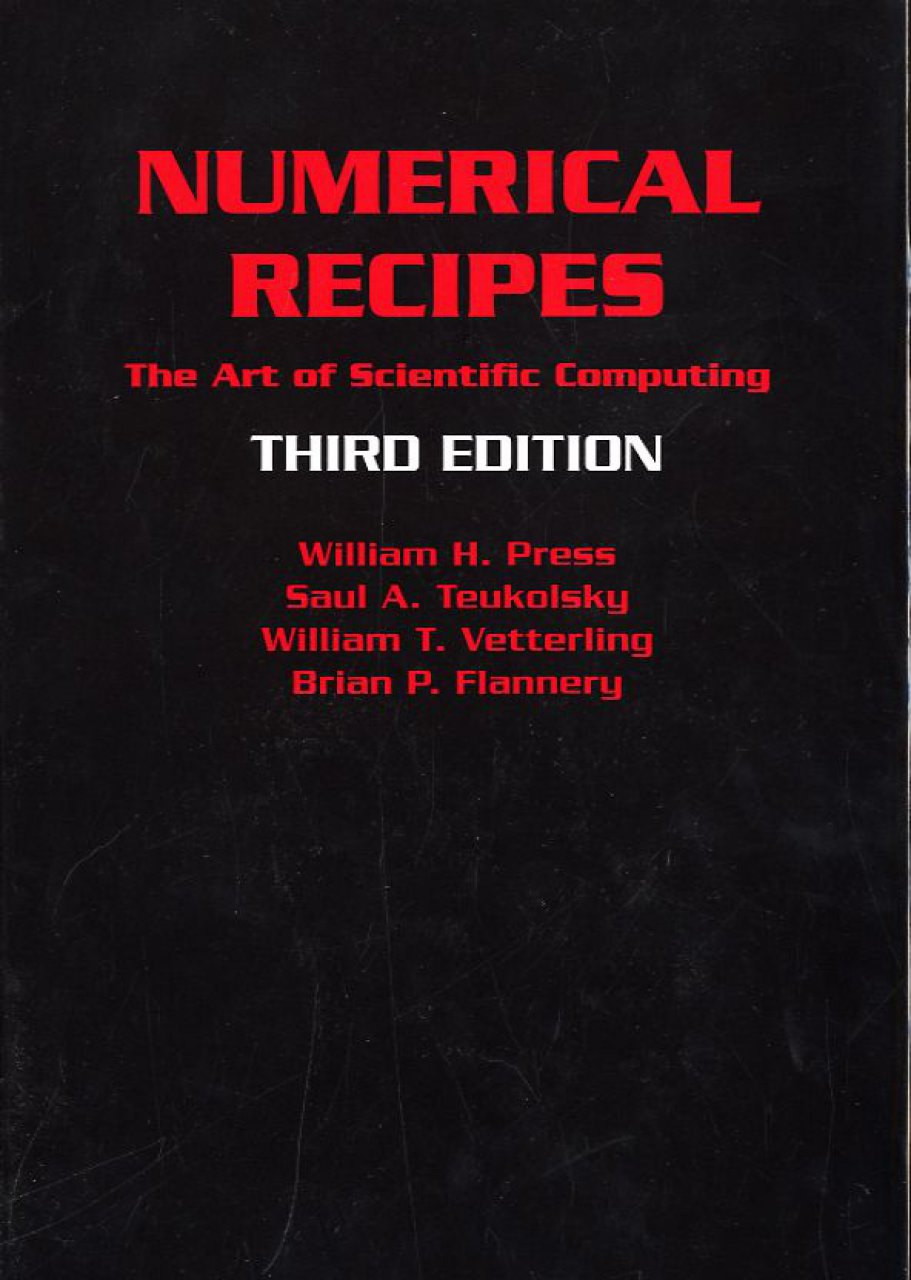
\includegraphics[width=1\textwidth]{img/numericalrecipes}
  \end{columns}
\end{frame}

\section{Big Numbers}
\subsection{Why big numbers}

\begin{frame}
  \frametitle{Big numbers in computers}
  \begin{block}{}
    When we talk about \structure{Big Numbers}, we usually mean large
    integers. Programming languages usually have primitive variables
    with a fixed number of bits. What is the biggest number that we
    can represent using this amount of bits?
  \end{block}
  
  \bigskip

  \begin{itemize}
    \item 32 bits: $2.147.483.648$
    \item 64 bits: $9.223.372.036.854.775.808$
    \item 128 bits: $1.701331*10^{38}$
  \end{itemize}
\end{frame}

\begin{frame}
  \frametitle{How big is big enough?}

    \begin{itemize}
    \item 32 bits: $2.147.483.648$
    \item 64 bits: $9.223.372.036.854.775.808$
    \item 128 bits: $1.701331*10^{38}$
    \end{itemize}

    \begin{block}{Where can we use these?}
    \end{block}
    
    \begin{itemize}
    \item Speed of Light: 300.000 m/s;
    \item<2-> Closest star system (5 light years):\\ $47.304.000.000.000$ km; 
    \item<3-> Number of atoms in the universe: $1*10^{80} atoms$;
    \item<4-> Digits of pi: more than $1*10^{100.000.000}$;\\
      \alert{damn mathematicians!}
    \end{itemize}    
\end{frame}

\begin{frame}
  \frametitle{Size and Precision}
  \begin{block}{}
    By using the correct representation, we can store numbers of any
    size in a fixed length integer:
  \end{block}

  \bigskip

  \begin{itemize}
  \item $47.304.000.000.000$ km -> $4.7304{+e}13$ km    
  \end{itemize}
  
  \bigskip

  {\small
  \begin{block}{}
    However, our \structure{precision} is limited:
  \end{block}}

  {\small
  \begin{itemize}
  \item $47.304.000.000.000$ km -> $4.7304{+e}13$ km
  \item $47.304.000.013.200$ km -> $4.7304{+e}13$ km
  \item $47.304.005.037.001$ km -> $4.7304{+e}13$ km
  \end{itemize}}
\end{frame}

\begin{frame}
  \frametitle{Don't forget your libraries!}
  \begin{itemize}
    \item \structure{C++}: \emph{Integer} class
    \item \structure{Java}: \emph{java.math.BigInteger} class
  \end{itemize}
  \bigskip

  Many programming languages provide support for big intergers ``Out
  of the Box''. Sometimes it may be necessary to make your
  implementation of big integers, but keep these classes in mind!
\end{frame}

\subsection{Representation}
\begin{frame}
  \frametitle{How to represent big Integers (1)}

  \begin{block}{Array of Digits}
    \begin{itemize}
    \item Very simple to implement;
    \item First element of the array is the least significant digit;
    \item Keep the index of the last digit at hand;
    \end{itemize}
  \end{block}
  
  \begin{block}{Linked List of Digits}
    \begin{itemize}
    \item Since each item is just a digit, you occupy double the space with pointers.
    \item If you have few big numbers, but many small ones, this saves some memory.
    \end{itemize}
  \end{block}
\end{frame}

\begin{frame}
  \frametitle{How to represent big Integers (2)}
  \begin{block}{What base should we use?}
    \begin{itemize}
    \item A decimal base sounds natural, but not required!
    \item A higher base means we need fewer digits (smaller arrays)
      \begin{itemize}
      \item Example: Octal base (base 8), Hexadecimal base (base 16)
      \end{itemize}
    \item On the other hand, you need extra functions to transform the numbers;
    \end{itemize}
  \end{block}
  
  \begin{block}{Pay attention to the sign!}
    \begin{itemize}
    \item You will need to keep an explicit field for the number's
      sign;
    \item This creates a special case: -0 and +0 are different!
    \item Don't forget to transform -0 numbers into +0 in your operators;
    \end{itemize}
  \end{block}
\end{frame}

\subsection{Operations}

\begin{frame}
  \frametitle{BigNum Operations} 

  Traditional arithmetic operations in big numbers are not different
  from what we know. However, there are a number of caveats that occur
  because:
  \begin{itemize}
  \item We are operating on one digit at a time;
  \item We are explicitly dealing with the sign;
  \item We want to be efficient;
  \end{itemize}
\end{frame}

\begin{frame}
  \frametitle{Addition (a,b)}
  
  Start the addition digit by digit, starting from the least
  significant. Any overflow should be added as a carry to the next
  digit

  \bigskip

  \begin{block}{Caveats}
    \begin{itemize}
    \item If $a$ and $b$ have different signs, it becomes a
      subtraction. Switch the sign of the parameter and send it to the
      subtraction function!
    \item Don't forget that the carry may add an extra digit to the
      final result!
    \end{itemize}
  \end{block}
\end{frame}

%% Subtraction: Normal Method
\begin{frame}
  \frametitle{Subtracting (borrow method)}
  
  Subtract each digit, starting from the least significant. If the
  result is negative, add \emph{base} and increment a \emph{borrow}
  counter. This counter is subtracted from the next digit.

  \bigskip

  \begin{block}{Caveats}
    \begin{itemize}
    \item Order the parameters by their most significant digit, to
      avoid special cases when borrowing;
    \item Ordering the parameters also avoids having to decide what is
      the final sign;
    \item Don't forget to adjust zeroes, and deal with -0;
    \end{itemize}
  \end{block}
\end{frame}


%% Subtraction: Complement
\begin{frame}
  \frametitle{Subtracting (complement method)} 

  We can use the \structure{complement} of the base to make
  subtraction using only additions.

  This makes more sense in the machine code level, because the
  complement of base 2 has many useful properties. But it can also be
  done at higher bases.
  
  \bigskip

  \begin{block}{caveats}
    \begin{itemize}
    \item You need to either order the numbers, to always subtract the
      smaller from the larger;
    \item Or you need to check for carry, to complement the result
      again in case it underflows;
    \item Don't forget to add 1 in the regular case!
    \end{itemize}
  \end{block}
\end{frame}


%% Multiplication
\begin{frame}[fragile,singleslide]
  \frametitle{Multiplication} 

  \begin{block}{}
  A simple way to implement multiplication is to use the traditional
  method that we learn at school:
  \end{block}
  
\begin{columns}[c]
  \column{0.5\textwidth}
\begin{verbatim}
  1234
   312 x
  ======
  1234*2 +
 12340*1 +
123400*3
========
\end{verbatim}
\column{0.5\textwidth}
\begin{verbatim}
  1234 +
  1234 +
 12340 +
123400 +
123400 +
123400
========
\end{verbatim}
\end{columns}
\end{frame}

\begin{frame}[fragile,singleslide]
  \frametitle{Multiplication}
  \begin{block}{Schoolhouse Multiplication}
{\smaller
\begin{verbatim}
multiply_bignum(bignum *a, bignum *b, bignum *c) {
  bignum row; /* represent shifted row */
  bignum tmp; /* placeholder bignum */
  int i,j;    /* counters */
  row = *a;
  for (i=0; i<=b->lastdigit; i++) {
    for (j=1; j<=b->digits[i]; j++) {
      add_bignum(c,&row,&tmp);
      *c = tmp;
    }
    digit_shift(&row,1);
  }
  c->signbit = a->signbit * b->signbit;
}
\end{verbatim}}
  \end{block}
\end{frame}

\begin{frame}
  \frametitle{Fast Multiplication} 
  \begin{block}{Complexity}
    {\small
    Traditional multiplication on $n$ digits requires $O(n^2)$
    elementary operations. There are special algorithms that produce
    faster results for large numbers.}
  \end{block}
  \begin{block}{Karatsuba Method}
    {\small
    Breaks $a$ and $b$ into numbers with less digits ($a_0 *b^m +
    a_1$,$b_0 *b^m + a_2$), and multiply these numbers. This is done
    recursively. Complexity is $O(n^{\log_23})$}
  \end{block}
  \begin{block}{Schonhage-Strassen Algorithm}
    {\small 

      Uses Fast-Fourier Transform to get a complexity
      $O(n\log{n}\log\log{n})$. Only used in practice when the number
      of \emph{digits} is 30.000 or more.  
    }
  \end{block}
\end{frame}

\begin{frame}[fragile,singleslide]
  \frametitle{Division}
  \begin{block}{}
    Division can, in principle, be dealt in a similar way to
    multiplication. We repeatedly subtract the dividend, and then
    shift it to the right.
  \end{block}

  \begin{columns}[c]
    \column{0.5\textwidth}
\begin{verbatim}
  450203
      23 %
  ======
  230000*1 -
   23000*9 -
    2300*5 - 
     230*7 -
      23*4 -
  ======
       1   (19574)
\end{verbatim}
\column{0.5\textwidth}
  \end{columns}
\end{frame}


\begin{frame}
  \frametitle{Exponentiation}
  \begin{block}{}
    There is a neat trick to make fast exponentiation, do you remember it?
  \end{block}
  \begin{onlyenv}<2>
    \begin{block}{}
      Normally we approach exponentiation in a ``divide and conquer''
      fashion. Cache the partial answers, because they will repeat
      many times.
      \begin{itemize}
      \item $A^n = A^{floor(n/2)} * A^{floor(n/2)} * A^{(n(mod)2)}$
      \end{itemize}
    \end{block}
  \end{onlyenv}
\end{frame}

%%%%%%%%%%%%%%%%%%%%%%%%%%%%%%%%%%
\section{Small Numbers}
\subsection{Introduction}

\begin{frame}
  \frametitle{Real Numbers}
  \begin{block}{Pesky infinity}
    \begin{itemize}
    \item In Mathematics, there is always a number between $a$ and
      $b$: $\frac{a+b}{2}$:
    \item In Computers, there is a limit to our precision, so this is
      not always true;
    \item In the case of floats, this is \structure{often} not true!
    \end{itemize}
  \end{block}

  \bigskip
  
  $a = (x + y) + z$\\
  $b = x + (y + z)$\\

  \begin{block}{}
    $a == b$ may return false, if $a$ and $b$ are floats! :-(
  \end{block}
\end{frame}

\begin{frame}
  \frametitle{Types of Real Numbers}
  \begin{block}{Rational Numbers}
    Can be represented by $a/b$, where $a$ and $b$ are integers. In
    general it is easier to do all representation and operations
    directly on these integers.\\
    \structure{Note:} Every integer $c$ can be represented as $c/1$
  \end{block}
  \begin{block}{Irrational Numbers}
    Some Real numbers can't be represented as a fraction of two
    integers. For example, $\pi$, $e$, $\sqrt{2}$, etc. Like with
    large integer, there is a limit to the precision of these numbers
    which depends on the number of digits that we can store.
  \end{block}
\end{frame}

\begin{frame}
  \frametitle{Representing Real Numbers} 

  Floating point numbers in \emph{floats} and \emph{doubles} are
  represented using the IEEE notation:
  \smallskip

  \begin{center}
    $a*2^c$
  \end{center}
  \smallskip

  Where $a$ (the mantissa) and $c$ (the exponent) have a limited
  number of bits. This implies that making operations on numbers with
  very different exponents is a recipe for numerical imprecisions.
  \bigskip
  
  \begin{block}{Warning}
    Do not directly compare two floats using $==$ : there is
    frequently precision errors. Instead, you want to test if their
    differences lie whithin a limit $\epsilon$. Or just use integers.
  \end{block}
\end{frame}

\subsection{Operations}

\begin{frame}
  \frametitle{Operations on Rational Numbers}
  \begin{block}{}
    Given two rational numbers, $c = x_1/y_1$ and $d = x_2/y_2$, the
    basic arithmetic operations are easy to program:
  \end{block}
  \begin{itemize}
  \item Addition: $c+d = \frac{x_1y_2 + x_2y_1}{y_1y_2}$
  \item Subtraction: $c-d = \frac{x_1y_2 - x_2y_1}{y_1y_2}$
  \item Multiplication: $cd = \frac{x_1x_2}{y_1y_2}$
  \item Division: $c/d = \frac{x_1y_2}{x_2y_1}$
  \end{itemize}
  \begin{block}{Warning!}
    Repeating all these multiplications leads to a serious danger of
    overflows! \structure{Reduce the Fractions} from time to time to
    avoid this.
  \end{block}
  
\end{frame}

\section{Algebra}
\subsection{Polynomials}

\begin{frame}[singleframe,fragile]
  \frametitle{Polynomials}

  \begin{block}{}
    It is useful to think of univariate polynomials as a special case
    of Big Numbers. In this case, the \emph{base} of the big number is
    the variable, and the digits are the coefficients. (Except that
    there is no carry)
  \end{block}
  \vspace{1cm}

\begin{verbatim}
   Polynomial(x) = {c0,c1,c2,c3...cn}
\end{verbatim}


\end{frame}

\begin{frame}
  \frametitle{Operation on Polynomials}
  \begin{block}{Evaluation}
    Brute force evaluation costs $O(n^2)$ multiplications. We can
    reduce this to $O(n)$ by using Horner's rule:\\
    \medskip

    $(((c_nx + c_{n-1})x + c_{n-2})x + ...)x + c_0$
  \end{block}

  \begin{block}{Addition, Subtraction}
    These operate in the sabe way as bignum additions and
    subtractions, but without the carry/borrow.
  \end{block}
\end{frame}

\begin{frame}
  \frametitle{Operations on Polynomials}
  \begin{block}{Multiplication}
    The product of $P(x)$ and $Q(x)$ is the combination of all items:
    \begin{center}
    $\sum_{i=0}\sum_{j=0} (c_ic_j)x^{i+j}$
    \end{center}
    This all against all operation is known as
    \structure{convolution}. The brute force complexity is $O(n^2)$,
    but it can be done in $O(n\log n)$ with a FFT. Other convolutions:
    String matching, digit addition, etc.
  \end{block}
  \begin{block}{Division}
    Division is not a closed operation for polynomials, and needs to
    be treated as a special case. For example:
    \begin{center}
      $P(x) = 2x; Q(x) = x^2+1; P(x)/Q(x)$
    \end{center}
    Is not a polynomial, but rather a \structure{fractional function}.
  \end{block}
\end{frame}

\subsection{Logarithms}

\begin{frame}
  \frametitle{Logarithms and exponential roots} 

  Remember the basic rules of logarithms and exponentiations:
  \begin{center}
    $\log{xy} = \log{x} + \log{y}$\\
    $\log{x^y} = y\log{x}$
  \end{center}
  We can use these to easily find fractional exponents:
  \begin{center}
    $a^b = \exp(\ln(a^b)) = \exp(b\ln(a))$\\
    $\sqrt{x} = x^{1/2} = \exp(0.5\ln(x))$
  \end{center}
  Just beware of computational uncertainties!
\end{frame}


%%%%%%%%%%%%%%%%%%%%%%%%%%%%%%%%%%
\section{Problems}
\subsection{Next Week's Problems:}
\begin{frame}
  \frametitle{Problems for this week}
  \begin{itemize}
  \item Primary Arithmetic
  \item Reverse and Add
  \item Polynomial Coefficient
  \item Stern Brocot Number System
  \end{itemize}
\end{frame}

\end{document}
